\subsection{Subpaso 5-A: Seleccionar hora}
\begin{enumerate}
	\item Seleccione el intervalo de tiempo del día elegido para la reservación en la interfaz
    \textbf{IUGS-04 Seleccionar hora} de las disponibles.
\item Seleccione la hora inicial dentro del intervalo elegido.
\item Seleccione la hora final dentro del intervalo elegido.
\item Presione el botón \textbf{Aceptar}
\begin{figure}[hbtp]
	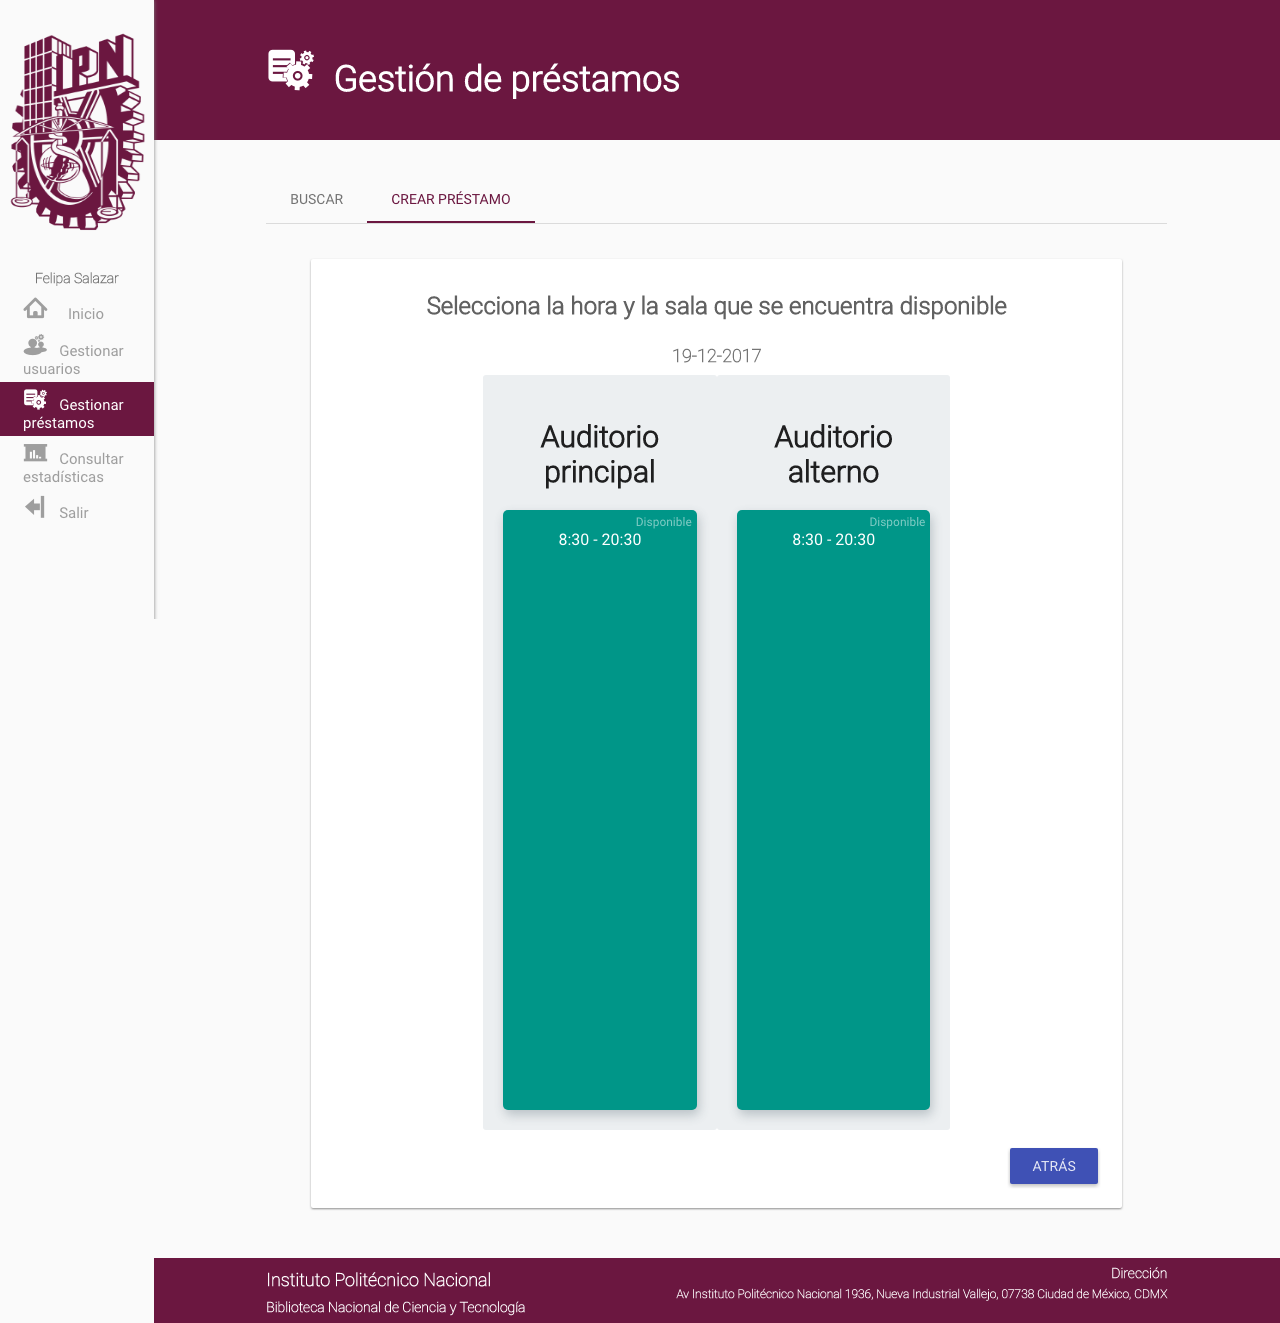
\includegraphics[scale=0.3]{images/Interfaz/IUGS-04 Seleccionar hora.png}
	\caption{Seleccionar hora}
	\end{figure}
\end{enumerate}

\subsection{Subpaso 5-B: Hora inválida}
\begin{enumerate}
	\item Seleccione la opción de \textbf{Aceptar} del mensaje
\textbf{MAT-56 Hora inválida}.
\item Seleccione nuevamente el intervalo de tiempo.
\begin{figure}[hbtp]
	\includegraphics[scale=0.3]{images/Interfaz/MAT-56 Hora inválida.png}
	\caption{Hora inválida}
	\end{figure}
\end{enumerate}

\subsection{Subpaso 5-C: Hora de inicio inválida}
\begin{enumerate}
	\item Seleccione la opción de \textbf{Aceptar} del mensaje
\textbf{MAT-54 Hora de inicio de préstamo inválida}.
\item Seleccione nuevamente la hora inicial dentro del intervalo elegido.
\begin{figure}[hbtp]
	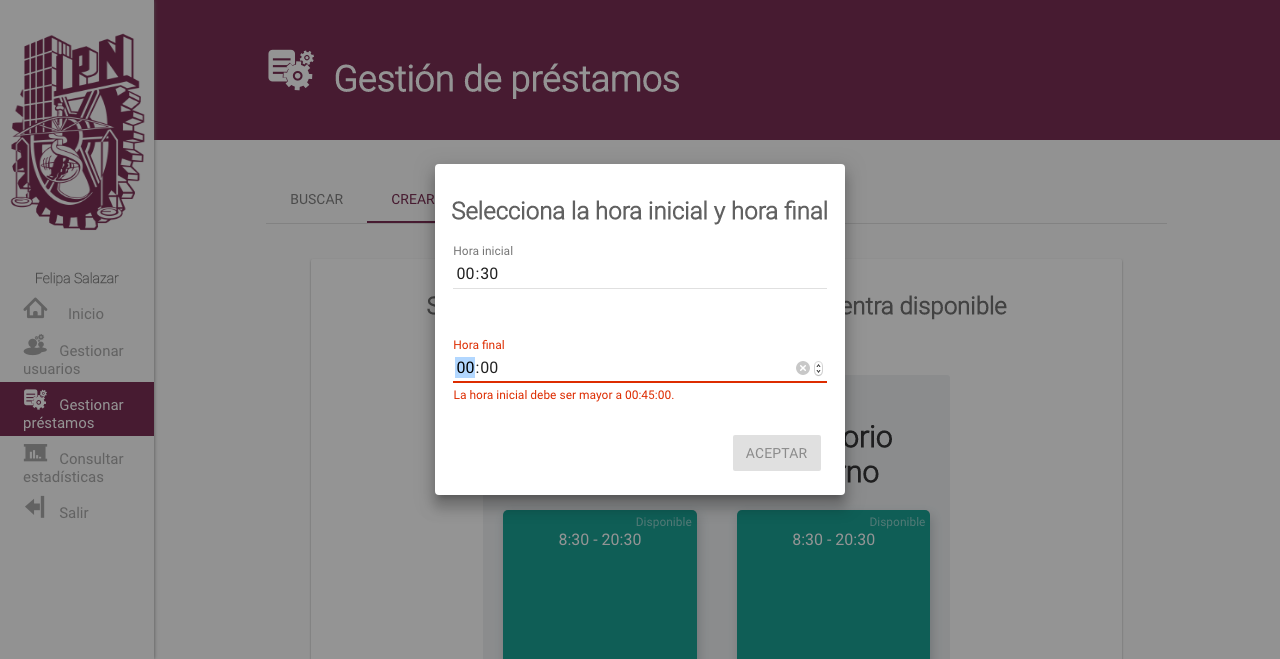
\includegraphics[scale=0.3]{images/Interfaz/MAT-54 Hora de inicio de préstamo inválida.png}
	\caption{Hora de inicio de préstamo inválida}
	\end{figure}
\end{enumerate}

\subsection{Subpaso 5-D: Hora de fin inválida}
\begin{enumerate}
	\item Seleccione la opción de \textbf{Aceptar} del mensaje
\textbf{MAT-55 Hora de fin de préstamo inválida}.
\item Seleccione nuevamente la hora final dentro del intervalo elegido.
\begin{figure}[hbtp]
	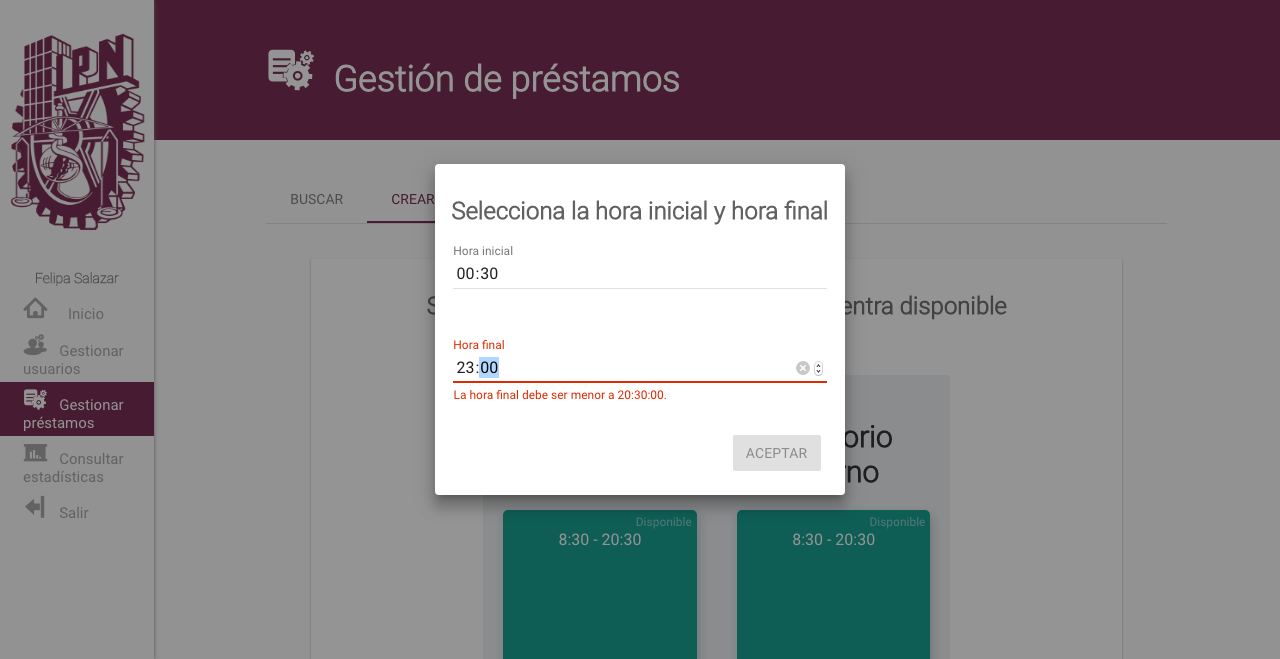
\includegraphics[scale=0.3]{images/Interfaz/MAT-55 Hora de fin de préstamo inválida.png}
	\caption{Hora de fin de préstamo inválida}
	\end{figure}
\end{enumerate}

\subsection{Subpaso 5-E: Campos incompletos}
\begin{enumerate}
	\item Seleccione la opción de \textbf{Aceptar} del mensaje
\textbf{MAT-18 Datos incompletos}.
	\item Llene todos los campos vacíos.
		  \begin{figure}[hbtp]
	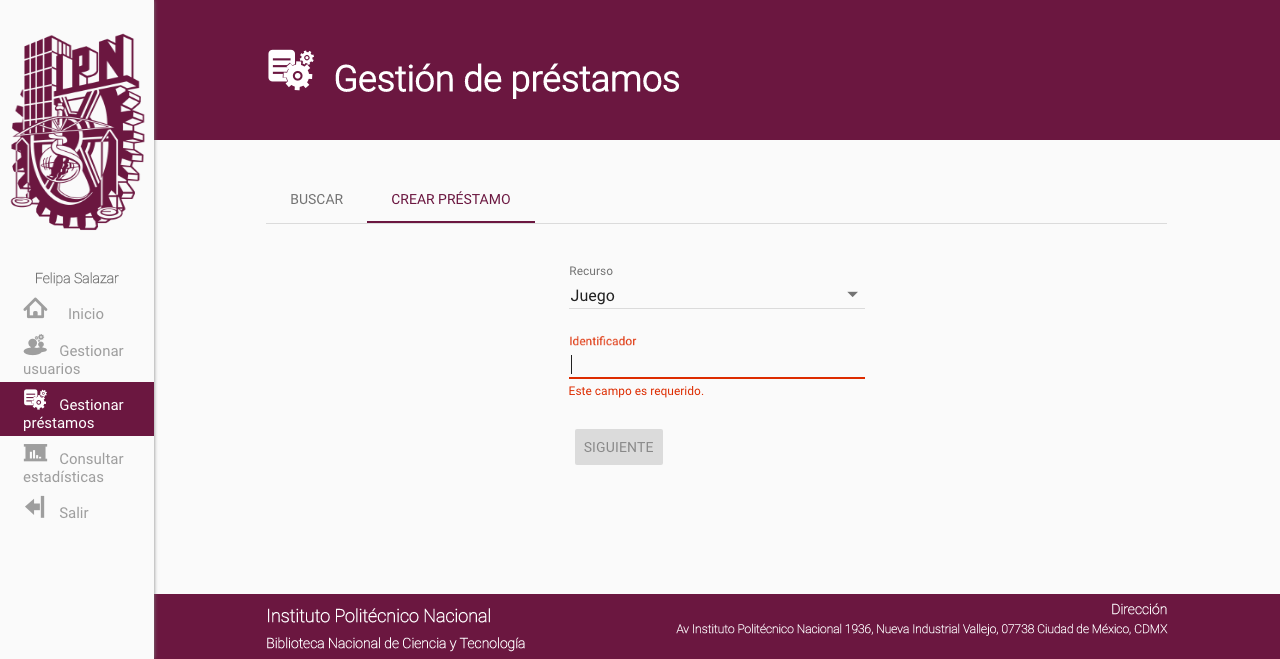
\includegraphics[scale=0.3]{images/Interfaz/MAT-18 Datos incompletos.png}
	\caption{Datos incompletos}
	\end{figure}
\end{enumerate}
